\documentclass[12pt,a4paper, xcolor=table]{article}
\usepackage{graphicx}
\usepackage[utf8]{inputenc}
\usepackage{eurosym}
\usepackage[spanish,es-tabla]{babel}
\usepackage[left=2cm, right=2cm, top=2cm, bottom=2cm]{geometry}
\usepackage{afterpage}
\PassOptionsToPackage{hyphens}{url}\usepackage{hyperref}
\usepackage{subfig}
\usepackage[table,xcdraw]{xcolor}


\usepackage{imakeidx}
\newcommand\blankpage{%
    \null
    \thispagestyle{empty}%
    \addtocounter{page}{-1}%
    \newpage}
\renewcommand*\contentsname{Índice: }

\makeindex
\let\olditemize\itemize
\def\itemize{\olditemize\itemsep=0pt}

\begin{document}
\setlength{\parindent}{0pt}
\begin{titlepage}
        \centering
        
\includegraphics[width=0.75\textwidth]{img/logo_uc3m.jpg}\par\vspace{3cm}
        {\huge\bfseries Práctica 1 \\ Aplicación de RNA\par}
        \vspace{0.5cm}
        {\scshape\Large Inteligencia Artificial en las Organizaciones\par}
        \vspace{1.5cm}
        {\scshape\Large Grupo 83\par}
        \vspace{1.5cm}
        {\Large\itshape Miguel Gutierrez Pérez\par}
        {\Large 100383537@alumnos.uc3m.es \par}
        \vspace{1cm}
        {\Large\itshape Mario Lozano Cortés\par}
        {\Large 100383511@alumnos.uc3m.es\par}
        \vspace{1cm}
        {\Large\itshape Alba Reinders Sánchez\par}
        {\Large 100383444@alumnos.uc3m.es\par}
        \vspace{1cm}
        {\Large\itshape Alejandro Valverde Mahou\par}
        {\Large 100383383@alumnos.uc3m.es\par}
        \vfill

% Bottom of the page
        {\large \today\par}
\end{titlepage}

\tableofcontents

\newpage

\section{Introducción}
    
\section{Parte 1: Aproximación usando Weka}

    \subsection{Planteamiento y desarrollo del problema a tratar}
    
    El objetivo de la asignatura de Inteligencia Artificial en las Organizaciones es el poner en relieve el encaje de las diversas técnicas de IA en contextos reales. Con esta motivación en mente, parece evidente que es imprescindible lograr obtener soluciones a problemas apremiantes con el conjunto de técnicas disponibles. Por su parte, la \textbf{epidemia} del\textbf{ SARS-CoV-2 }supone un \textbf{reto} para la humanidad y constituye una oportunidad para demostrar el potencial de las nuevas herramientas IA de las que disponemos para hacer frente a este nuevo reto.

    \vspace{2mm}
    
    Uno de los \textbf{modelos computacionales} cuya \textbf{aplicación} resulta \textbf{atractiva} es el de las Redes de Neuronas Artificiales. La capacidad de aprender de grandes conjuntos de datos hacen de esta una opción perfecta para comprender y predecir los contagios causados por el virus. 
    
    Para comprender cómo cumplir con este objetivo debemos tener en cuenta cómo es posible que una red de neuronas aprenda. La respuesta se haya en su estructura. A nivel básico la estructura de una RNA supone un conjunto de entradas multiplicadas por unos pesos a modo de impulso nervioso al que se le puede aplicar determinadas funciones de activación. Dicha estructura de una neurona puede ser vista a continuación.    
   
    \begin{figure}[h]
        \centering
        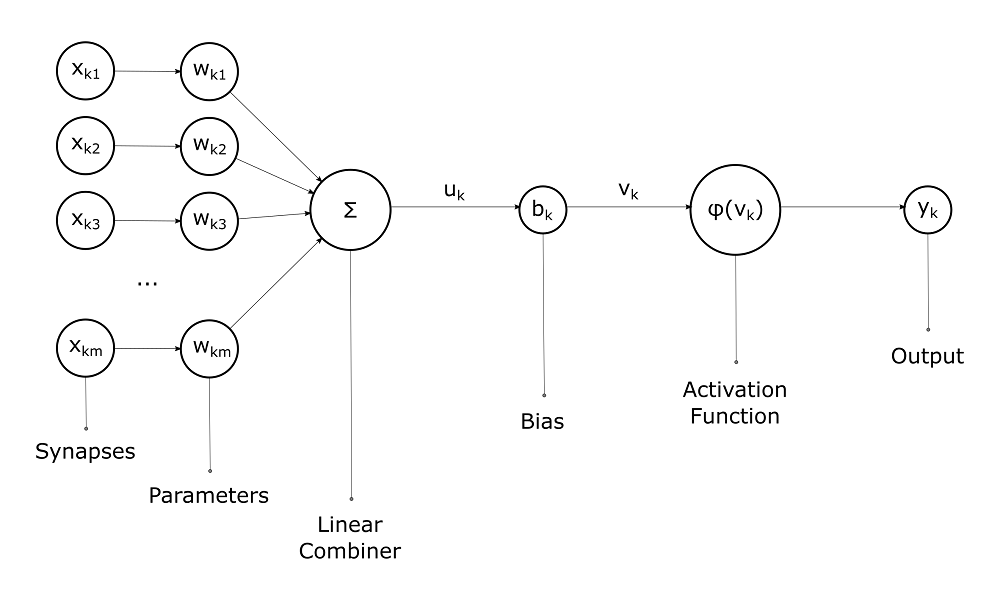
\includegraphics[width=400px]{img/Neuron.png}
        \caption{Estructura de una neurona}
        \label{fig:graf_exp1}
    \end{figure}

    Por lo tanto, hemos trasladado el problema a la \textbf{selección de los pesos} precisos para realizar predicciones lo más exactas posibles. El modelo a emplear se tratará del \textbf{Perceptrón Multicapa}. Consecuentemente el trabajo realizado en esta práctica consiste en \textit{tratar los datos para la aplicación del modelo elegido}, \textit{realizar los experimentos oportunos para dar con una configuración de la red apropiada} y \textit{analizar los resultados} obtenidos haciendo una reflexión crítica del proceso seguido.
        
    \newpage

    \subsection{Tratamiento de datos}

    Los datos que se han utilizado pertenecen al \textit{Novel Coronavirus (COVID-19) Cases Data} de la página \textit{The Humanitarian Data Exchange}, se trata de una recopilación de \textbf{datos epidemiológicos del COVID-19} desde el día 22 de enero de 2020.

    \vspace{3mm}

    En concreto, los datos de interés son los que se encuentran en el fichero diario de casos confirmados, este está compuesto de \textbf{266} provincias/estados de distintos países/regiones, de los cuales se recopila el \textbf{número de infectados totales} desde el 22 de enero hasta la fecha.  

    \vspace{1mm}

    Los primeros atributos son: nombre de la provincia/estado, país/región, longitud y latitud (del país). Seguidos del número de contagiados acumulados por día.

    \vspace{3mm}

    El tratamiento de los datos que se ha llevado a cabo es el siguiente:

    \begin{itemize}
        \item En primer lugar, se ha eliminado la comilla simple del nombre de un país del fichero, para evitar errores en \textit{Weka}.
        \item Se han renombrado los atributos correspondientes a las fechas para que el fichero sea compatible con nuevos datos, para ello se renombra el día actual a \textit{Día 0} y el resto a \textit{Día -1}, \textit{Día -2},\dots
        \item Por último, se convierte el fichero \textit{.csv} en \textit{.arff}.
    \end{itemize}

    Además, se ha generado un nuevo fichero para abordar la generación de resultados sobre los territorios concretos en los que se focaliza la atención de la práctica, \textbf{Brasil} y \textbf{España}. Dicho fichero se obtiene borrando del fichero \textit{.arff} anterior las filas que no corresponden a estos países.

    \subsection{Configuración de experimentos con MLP}

    \subsection{Análisis de resultados}

\section{Parte 2: }

\section{Contexto de la práctica}


 \section{Conclusiones}

\clearpage 

\section{Referencias}
    \begin{itemize}
        \item [1.] Introduction to Neurons in Neural Networks. Medium. Consultado en Octubre 2020. Url: \\
        \href{https://medium.com/artificial-neural-networks/introduction-to-neurons-in-neural-networks-71828d040a65}{https://medium.com/artificial-neural-networks}
    \end{itemize}
\printindex
\end{document}
